\section{ETMS}

Através da interface do \textit{Central Management} é possível efectuar as configurações necessárias ao funcionamento do servidor de email \footnote{O sistema foi implementado de modo a manter a compatibilidade com o \textit{Webmin}.}.

A gestão divide-se em três separadores, respeitantes a diferentes contextos de configuração. O primeiro separador indica o estado do serviço e permite iniciar, parar ou reiniciar o serviço. É também possível efectuar \textit{backups} da sua configuração (no próprio agente) e o restauro da mesma - útil para testar novas configurações. No segundo separador pode ser efectuada a configuração de de domínios. Por último, o terceiro separador permite a configuração de contas de correio. As sub-secções \ref{sec:etms_gerir_dominios} e \ref{sec:etms_sub_gerir_caixas_dominio} indicam as possíveis configurações. 

A imagem \ref{fig:etms_main_info} ilustra os separadores existentes. Para os encontrar seleccione a máquina virtual que contém a instalação do \textit{ETMS}, seguido da opção \textit{ETMS} que se encontra nos separadores do painel do lado direito.


\begin{figure}[H]
    \begin{center}
    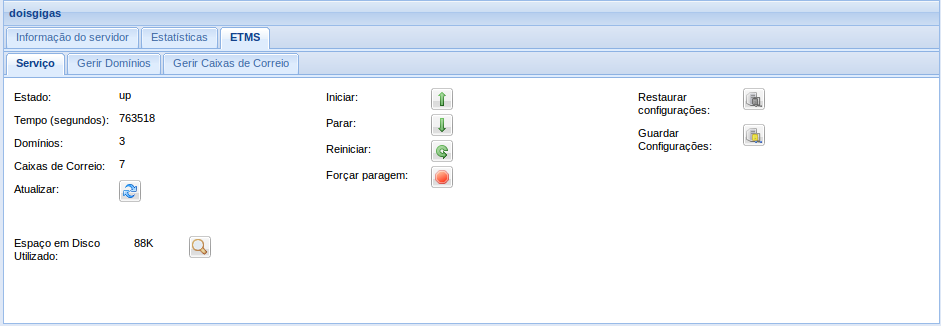
\includegraphics[scale=0.38]{screenshots/etms/etms_main_info.png}
    \caption{ETMS - Painel de Informação Principal}
    \label{fig:etms_main_info}
    \end{center}
\end{figure}


\subsection{Separador 1 - Serviço}
\label{sec:etms_info_principal}

O separador \textit{Serviço} está dividido em três colunas (imagem \ref{fig:etms_main_info}). À esquerda são indicadas informações sobre o processo que executa o serviço, nomeadamente: informação sobre o seu estado (\textit{Up} - a funcionar; \textit{Down} - parado), tempo no presente estado, o número de domínios e contas de correio existentes, e o espaço total ocupado pelos emails existentes no servidor. Note que o espaço total ocupado não fica visível logo após a abertura do separador, por se tratar de uma operação potencialmente demorada. Assim, para solicitar esta informação deve seleccionar o ícone à direita. A informação sobre o estado do serviço, é actualizada na primeira vez que o separador é aberto, podendo ser refrescada sempre que solicitada de forma explicita, através da opção \textit{Actualizar}.

Na coluna central encontram-se opções para \textit{Iniciar}, \textit{Parar} e \textit{Reiniciar} o processo que suporta o serviço. Na eventualidade de haver dificuldade em parar o serviço a opção \textit{forçar paragem} deve ser utilizada.

Na coluna à direita estão definidas as operações de \textit{Backup} e \textit{Restauro das Configurações}. Estas opções \textbf{devem apenas} ser utilizadas no teste de novas configurações, pois o seu armazenamento é efectuado localmente (na maquina onde se encontra o servidor de email).

\subsection{Separador 2 - Gerir Domínios}
\label{sec:etms_gerir_dominios}

O conteúdo do separador \textit{Gerir Domínios} é dividido em duas áreas/grelhas, onde é possível seleccionar linhas (imagem \ref{fig:etms_criar_dominio_1}). A grelha da esquerda indica quais os domínios existentes, a da direita, lista os \textit{Alias} existentes para o domínio seleccionado.

Em ambas as áreas é possível efectuar operações sobre o item seleccionado, através da utilização dos botões disponíveis na barra de ferramentas sob a grelha em questão. Note que ao seleccionar um domínio a lista de \textit{alias} é actualizada e substituída para o domínio em questão.

\begin{figure}[H]
    \begin{center}
    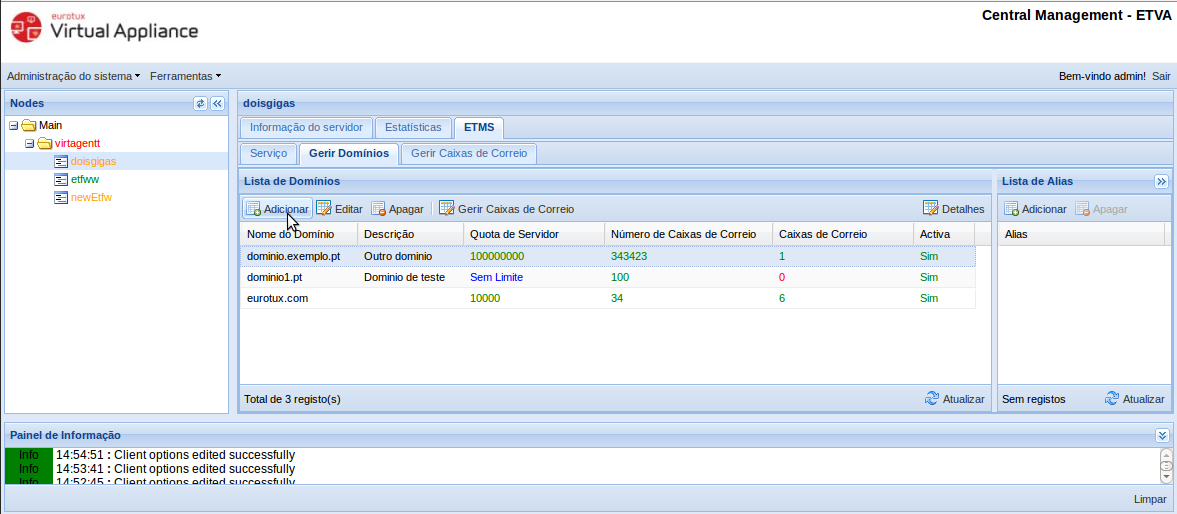
\includegraphics[scale=0.35]{screenshots/etms/etms_criar_dominio_1.png}
    \caption{ETMS - Painel de Gestão de Domínios}
    \label{fig:etms_criar_dominio_1}
    \end{center}
\end{figure}

\subsubsection{Criação de um Domínio}
\label{sec:etms_sub_criacao_dominio}

Para criar um domínio utilizar a opção \textit{Adicionar}, onde de seguida se abrirá uma janela com os campos a preencher, como ilustra a figura \ref{fig:etms_criar_dominio_2}. Após preencher os campos seleccionar \textit{Guardar} para efectuar a alteração. Note que: os três primeiros campos são de carácter obrigatório; a grelha com os domínios existentes é refrescada após a adição do novo domínio.

\begin{figure}[H]
    \begin{center}
    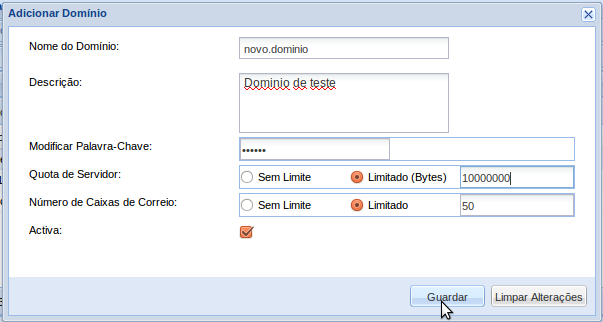
\includegraphics[scale=0.35]{screenshots/etms/etms_criar_dominio_2.png}
    \caption{Criar Domínio}
    \label{fig:etms_criar_dominio_2}
    \end{center}
\end{figure}

Para uma melhor compreensão, descrevem-se sucintamente os campos existentes, indicando para cada um exemplo:
\begin{itemize}
\item \textbf{Nome do Domínio} - Qual o nome do domínio pretendido (Ex: eurotux.com)
\item \textbf{Descrição} - Breve descrição sobre o domínio (Ex: Tecnologias de Informação)
\item \textbf{Palavra-Chave} - \textit{Password} a utilizar na gestão do domínio\footnote{Para utilizadores do Webmin}, maior que seis caracteres. (Ex: PassWord)
\item \textbf{Quota de Servidor} - Valor máximo a utilizar no armazenamento de emails(Ex: 1000000000 Bytes)
\item \textbf{Número de Caixas de Correio} - Número limite de caixas de correio que podem ser definidas para o domínio. Note que este campo pode impedir a criação de novas caixas. Porém a redução do seu valor não elimina contas previamente criadas. (Ex: 10)
\item \textbf{Activo} Indica se o serviço está activo para o domínio seleccionado. Na realidade esta opcção altera o estado das contas de email, inibindo ou não a entrega de novas mensagens.
\end{itemize}

\subsubsection{Edição de um Domínio}
\label{sec:etms_sub_edicao_dominio}
Para editar um domínio, seleccionar a linha correspondente, e escolher a opção \textbf{Editar}. Abrir-se-á uma janela (ver figura \ref{fig:etms_criar_dominio_2}) com os atributos do domínio, referidos anteriormente mas preenchidos com as configurações previamente efectuadas (subsecção anterior \ref{sec:etms_sub_criacao_dominio}). 

Após guardar, a grelha que lista os domínios existentes é actualizada com as novas configurações.

\subsubsection{Remoção de um Domínio}
\label{sec:etms_sub_remocao_dominio}
A remoção de um domínio implica também a remoção dos \textit{Alias} e contas de correio associadas (incluindo emails existentes, não sendo possível recupera-los através do processo de restauro de configurações). Para a remoção de um domínio, seleccionar a linha que identifica o domínio a remover, e escolher a opção \textbf{Apagar}. De seguida responder afirmativamente à questão que confirma a operação, como ilustra a imagem \ref{fig:etms_delete_domain}. O sucesso da operação é indicado no \textit{Painel de Informação}.

\begin{figure}[H]
    \begin{center}
    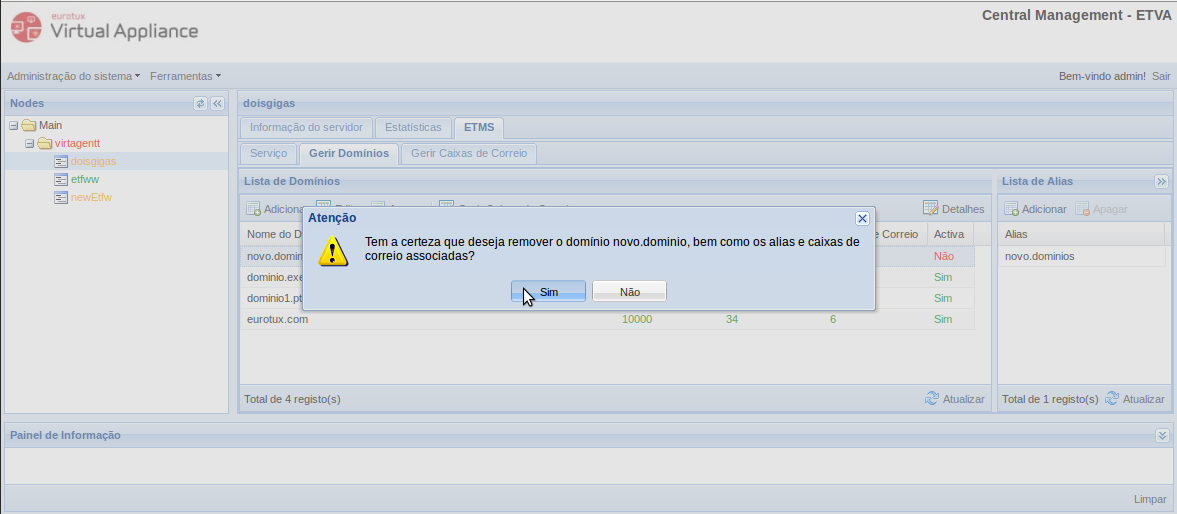
\includegraphics[scale=0.35]{screenshots/etms/etms_delete_domain.png}
    \caption{Remover Domínio}
    \label{fig:etms_delete_domain}
    \end{center}
\end{figure}


\subsection{Gerir Caixas de Correio}
\label{sec:etms_sub_gerir_caixas_dominio}
A opção \textit{Gerir Caixas de Correio} facilita a alteração das caixas de correio do domínio. Ao seleccionar esta opção é encaminhado automaticamente para o separador \textit{Gerir Caixas de Correio}, e é efectuada uma pesquisa por caixas de correio pertencentes ao domínio (ver imagem \ref{fig:etms_gerir_mailboxes}). Note que a opção \textit{Gerir Caixas de Correio} apenas fica visível se um domínio estiver seleccionado.

\begin{figure}[H]
    \begin{center}
    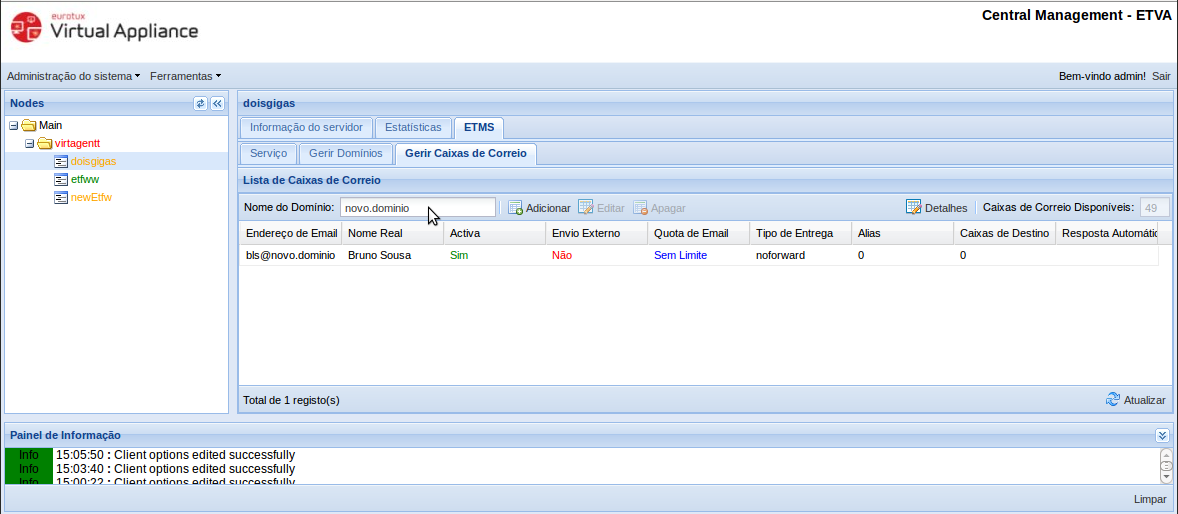
\includegraphics[scale=0.35]{screenshots/etms/etms_gerir_mailboxes.png}
    \caption{Gerir Caixas de Correio de um Domínio}
    \label{fig:etms_gerir_mailboxes}
    \end{center}
\end{figure}

\subsubsection{Opção Detalhes}
\label{sec:etms_sub_detalhes_dominio}
A opção \textit{Detalhes}, pertencente à barra de ferramentas que se encontra sob a \textit{Lista de Domínios} (à direita). Ao seleccionar esta opção é acrescentada uma coluna à grelha que lista os domínios, com informação sobre o espaço que cada um ocupa no sistema (ver imagem \ref{fig:etms_domain_details}). Note que, por se tratar de uma operação computacional intensiva e potencialmente demorada, ao efectuar outro tipo de operações esta coluna desaparece. Assim, sempre que se pretender actualizar/ver o espaço em disco em uso, deve utilizar-se esta opção.

\begin{figure}[H]
    \begin{center}
    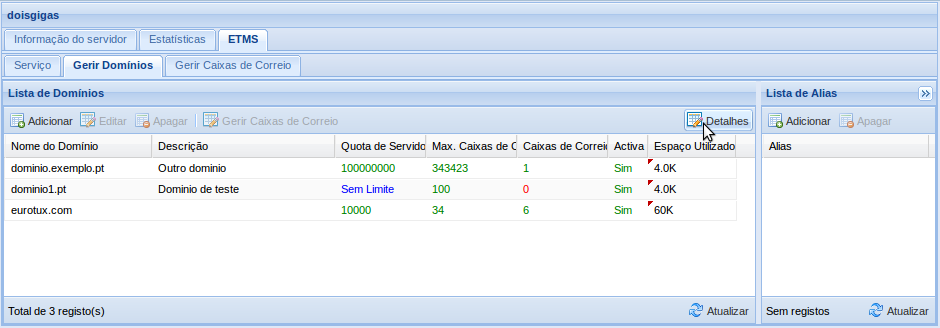
\includegraphics[scale=0.35]{screenshots/etms/etms_domain_details.png}
    \caption{Espaço Ocupado pelos Domínio}
    \label{fig:etms_domain_details}
    \end{center}
\end{figure}

\subsubsection{Criação de \textit{Alias}}
\label{sec:etms_sub_criacao_alias_dominio}
Para acrescentar um \textit{alias} a um domínio deve: seleccionar o domínio ao qual se pretendem adicionar \textit{alias}; na área da direita onde consta a \textit{Lista de Alias}, escolher a opção \textit{Adicionar}. Note que é acrescentada uma entrada ao início da lista, onde pode definir o novo \textit{alias} (ver figura \ref{fig:etms_criar_alias_dominio}). Quando seleccionar noutro local o novo \textit{alias} é enviado para o agente (ficando o canto superior esquerdo a vermelho durante esta operação). Se a operação for bem sucedida, é mostrada uma notificação \ref{fig:etms_criar_alias_dominio_success}, e acrescentada uma entrada ao \textit{Painel de Informação}.

\begin{figure}[H]
    \begin{center}
    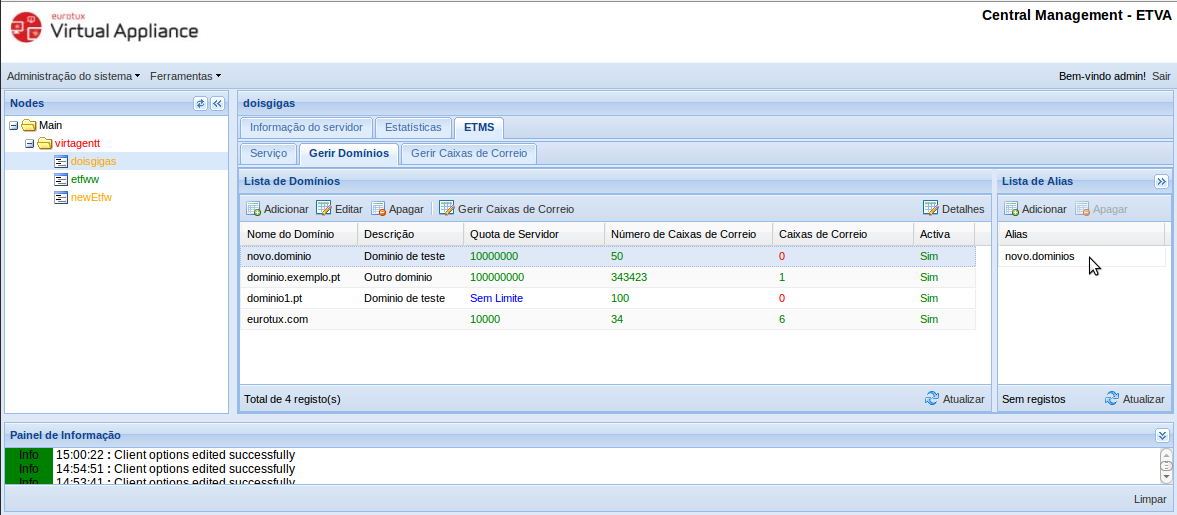
\includegraphics[scale=0.35]{screenshots/etms/etms_criar_alias_dominio.png}
    \caption{Adicionar Alias a um Domínio}
    \label{fig:etms_criar_alias_dominio}
    \end{center}
\end{figure}

\begin{figure}[H]
    \begin{center}
    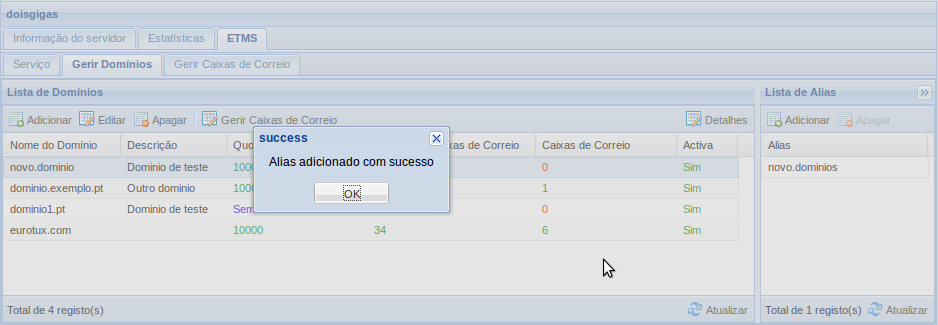
\includegraphics[scale=0.35]{screenshots/etms/etms_criar_alias_dominio_success.png}
    \caption{Sucesso na Criação de Alias de Domínio}
    \label{fig:etms_criar_alias_dominio_success}
    \end{center}
\end{figure}


\subsubsection{Remoção de \textit{Alias}}
\label{sec:etms_sub_remocao_alias_dominio}
Para remover um \textit{alias} deve: seleccionar o domínio que contém o \textit{alias} (imagem \ref{fig:etms_criar_alias_dominio}); à direita, na \textit{Lista de Alias}, seleccionar o alias que se pretende remover; Escolher a opção \textit{Apagar}; Responder afirmativamente à mensagem de confirmação.

Note que, sempre que necessário, a \textit{Lista de Alias} pode ser actualizada, através da barra de ferramentas inferior.

\subsection{Separador 3 - Gerir Caixas de Correio}
\label{sec:etms_caixas_correio}
O conteúdo do separador \textit{Gerir Caixas de Correio} consiste numa área/grelha, onde cada linha corresponde a uma caixa de correio (imagem \ref{fig:etms_gerir_mailboxes_mb}). As linhas da grelha são seleccionáveis e é possível efectuar operações sobre cada selecção. Para que a grelha seja preenchida é necessário efectuar uma pesquisa de caixas de correio, que pode ser efectuada seguindo os passos indicados em \ref{sec:etms_sub_pesquisar_caixas_correio}.

\begin{figure}[H]
    \begin{center}
    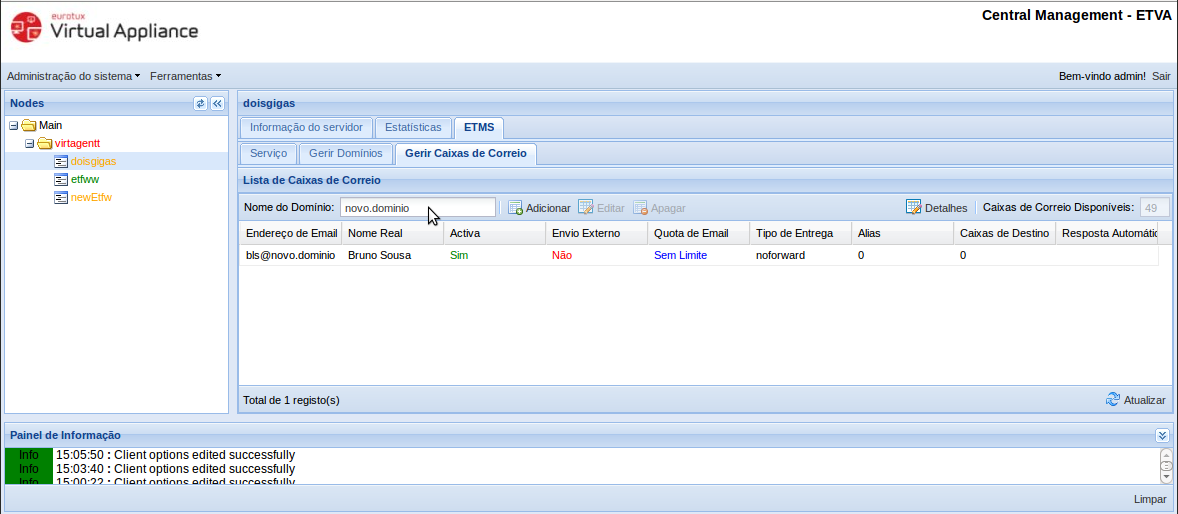
\includegraphics[scale=0.35]{screenshots/etms/etms_gerir_mailboxes.png}
    \caption{ETMS - Painel de Gestão de Caixas de Correio}
    \label{fig:etms_gerir_mailboxes_mb}
    \end{center}
\end{figure}


\subsubsection{Pesquisar Caixas de Correio}
\label{sec:etms_sub_pesquisar_caixas_correio}
É possível pesquisar pelas caixas de correio de determinado domínio, bastando para isso indicar o nome do domínio na caixa que fica sob a grelha (na barra de ferramentas), e premir \textit{ENTER}. A pesquisa é então efectuada. Repare que, durante o processo de comunicação com a máquina que aloja o serviço, o icone do canto inferior direito fica animado (perto da opção \textit{Actualizar}). Caso não seja encontrado o domínio, é apresentada uma mensagem de erro. A pesquisa com sucesso de um domínio, habilita as opções para gestão das caixas de correio (ver imagem \ref{fig:etms_gerir_mailboxes_mb}).

\subsubsection{Criação de uma Caixa de Correio}
\label{sec:etms_sub_criar_caixas_correio}
Para criar uma caixa de correio é necessário fazer uma pesquisa pelo domínio (ver \ref{sec:etms_sub_pesquisar_caixas_correio}), utilizar a opção \textbf{Adicionar} (abrir-se-á uma janela com os campos a preencher, como ilustra a figura \ref{fig:etms_criar_mailbox}), após preencher os campos seleccionar \textit{Guardar} para efectuar a alteração. Note que: os três primeiros campos são de carácter obrigatório; a grelha com os domínios existentes é refrescada após a adiçao do novo domínio.

\begin{figure}[H]
    \begin{center}
    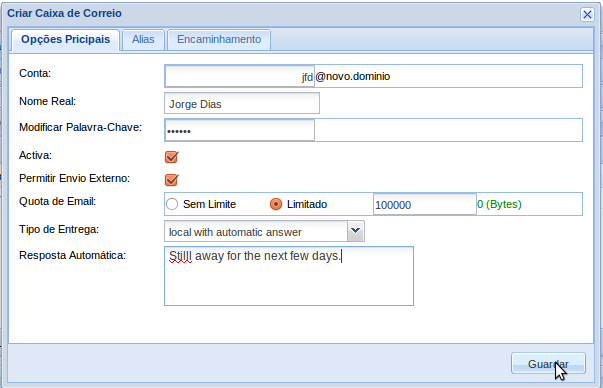
\includegraphics[scale=0.35]{screenshots/etms/etms_criar_mailbox.png}
    \caption{Criar Caixa de Correio}
    \label{fig:etms_criar_mailbox}
    \end{center}
\end{figure}

A janela de criação de uma nova caixa de correio é composta por três separadores: \textit{Opções Principais}; \textit{Alias} (ver subsecção \ref{sec:etms_sub_alias_caixas_correio}); \textit{Encaminhamento} (ver subsecção \ref{sec:etms_sub_encaminhamento_caixas_correio}).

Para uma melhor compreensão, descrevem-se sucintamente os campos existentes nas \textit{Opções Principais} indicando, sempre que oportuno, exemplos de utilização:
\begin{itemize}
\item \textbf{Conta} - Nome da conta pretendida (Ex: mfd@eurotux.com)
\item \textbf{Nome Real} - Nome do utilizador da conta \footnote{Para eventual necessidade de contacto} (Ex: Jorge Leal)
\item \textbf{Modificar Palavra-Chave} - \textit{Password} a utilizar na para aceder à caixa de correio\footnote{Para utilizadores do Webmin}, maior que seis caracteres. (Ex: PassWord)
\item \textbf{Activa} - Altera o estado da conta de email, inibindo/possibilitando a entrega de novas mensagens.
\item \textbf{Permitir Envio Externo} - Permitir à conta de email o envio de emails para fora do servidor, isto é, para domínios que não estejam definidos no servidor.
\item \textbf{Quota de Email} - Valor máximo a utilizar no armazenamento de emails. Note que à direita, a verde, é indicado o valor máximo definido para o domínio, não podendo a \textit{Quota de Email} exceder este valor (Ex: 10000 Bytes).
\item \textbf{Tipo de Entrega} - Existem quatro modos de entrega: local; encaminhado; local e encaminhado; local e encaminhado com resposta automática (ver imagem \ref{fig:etms_criar_alias_dominio_success}). Caso não seja seleccionado nenhum modo de encaminhamento, assume-se que o tipo de entrega é apenas local. Os modos de encaminhamento são descritos abaixo.
\item \textbf{Resposta Automática} - Mensagem com resposta automática, utilizada se o modo de entrega for \textit{Local com Resposta automática} (Ex: "Estou ausente")
\end{itemize}

Identificam-se os tipos de entrega possíveis:
\textit{Local} - Apenas é efectuada a entrega de emails na conta local, considerando-se também os \textit{alias} existentes para a conta.
\textit{Encaminhado} - Apenas é efectuada a entrega de emails para os emails definidos no separador \textit{Encaminhamento}.
\textit{Local e Encaminhado} - Os emails recebidos são entregues na caixa de correio local e encaminhados para os emails definidos no separador \textit{Encaminhamento}.
\textit{Local/Encaminhado com resposta automática} - Os emails são entregues na caixa local, encaminhados e é enviada uma mensagem para a origem do email, com o texto definido em \textit{Resposta Automática}.

\subsubsection{Edição de uma Caixa de Correio}
\label{sec:etms_sub_editar_caixas_correio}
A janela de edição de uma caixa de correio é semelhante à criação de novas caixas \ref{sec:etms_sub_criar_caixas_correio}, sendo que apenas é necessário seleccionar a caixa de correio que se pretende alterar, e escolher a opção \textit{Editar}. A diferença passa pelo facto do formulário ser automaticamente preenchido com as configurações da conta e o campo \textit{Modificar Palavra-Chave} fica por omissão desabilitado, sendo necessário seguir os passos em \ref{sec:etms_sub_password_caixas_correio} para proceder à sua alteração.


\subsubsection{Alterar a Palavra-Chave}
\label{sec:etms_sub_password_caixas_correio}
Para alterar a \textit{password} de determinada conta é necessário: seleccionar na grelha a conta pretendida; carregar em editar; na linha \textit{Modificar Palavra-Chave} seleccionar a caixa que lhe segue; definir a nova palavra-chave. Por último seleccionar guardar para terminar a configuração (ver imagem \ref{fig:etms_mb_pass_ed}).

\begin{figure}[H]
    \begin{center}
    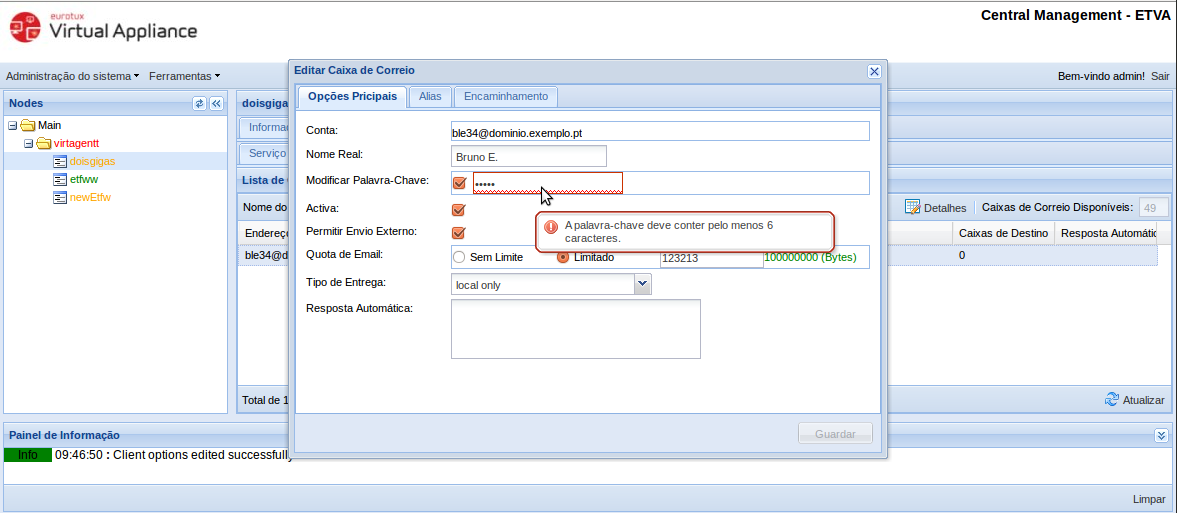
\includegraphics[scale=0.35]{screenshots/etms/etms_mb_pass_ed.png}
    \caption{Alerar Palavra-Chave de Caixa de Correio}
    \label{fig:etms_mb_pass_ed}
    \end{center}
\end{figure}

\subsubsection{Definição de Alias para a Caixa de Correio}
\label{sec:etms_sub_alias_caixas_correio}
Podem ser definidos \textit{alias} para caixas de correio existentes, bastando para isso acrescentar entradas na grelha \textit{Alias} no processo de criação/edição de uma caixa de correio (descrito em \ref{sec:etms_sub_criar_caixas_correio}). Note que \textbf{deve} ser indicado o email completo (ex: mfd.alias@eurotux.com), e que as alterações têm efeito após a selecção da opção guardar (ver imagem \ref{fig:etms_alias_create}).

\begin{figure}[H]
    \begin{center}
    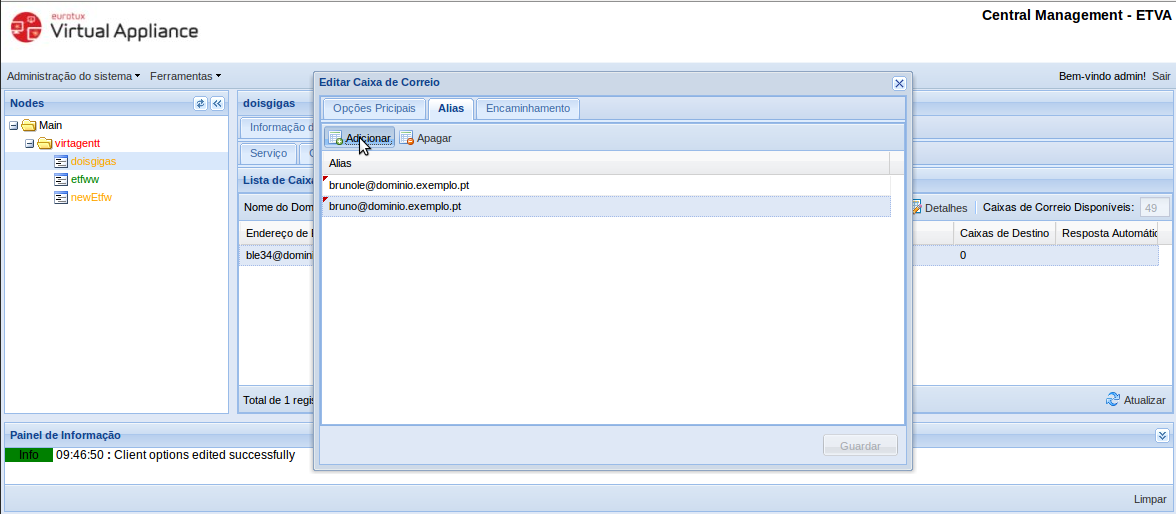
\includegraphics[scale=0.35]{screenshots/etms/etms_alias_create.png}
    \caption{Criar Alias para Caixa de Correio}
    \label{fig:etms_alias_create}
    \end{center}
\end{figure}

O procedimento para remover \textit{alias} passa por seleccionar o alias pretendido e escolher a opção \textit{Apagar}. Por último seleccionar \textit{Guardar} para que as alterações tenham efeito (ver imagens \ref{fig:etms_alias_mailbox_delete} e \ref{fig:etms_alias_mailbox_delete_2}).

\begin{figure}[H]
    \begin{center}
    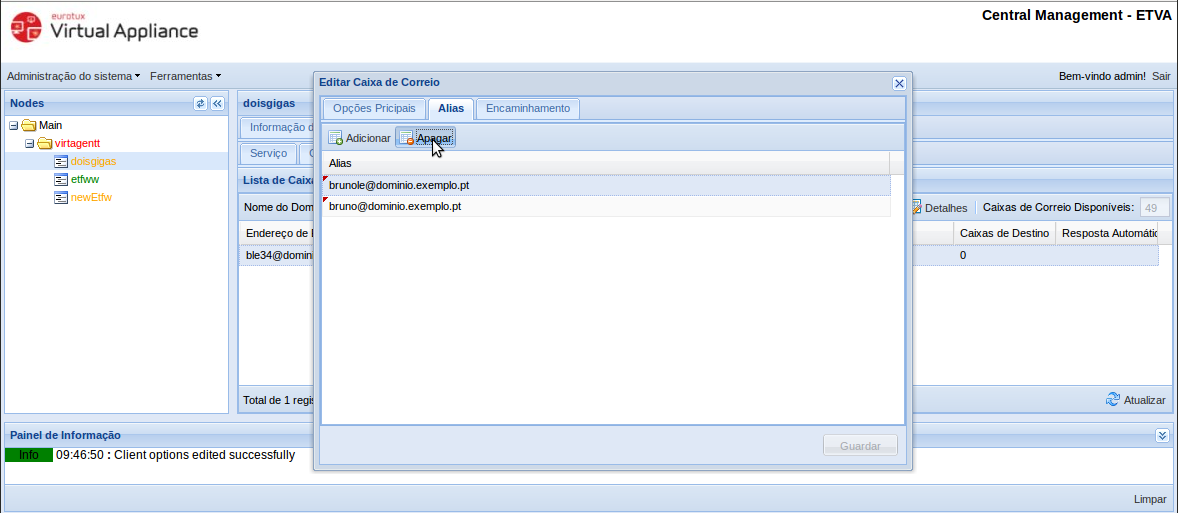
\includegraphics[scale=0.35]{screenshots/etms/etms_alias_mailbox_delete.png}
    \caption{Eliminar Alias de uma Caixa de Correio - passo 1}
    \label{fig:etms_alias_mailbox_delete}
    \end{center}
\end{figure}

\begin{figure}[H]
    \begin{center}
    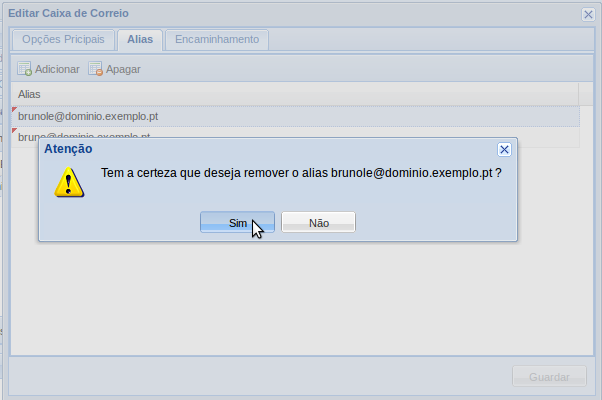
\includegraphics[scale=0.35]{screenshots/etms/etms_alias_mailbox_delete_2.png}
    \caption{Eliminar Alias de uma Caixa de Correio - passo 2}
    \label{fig:etms_alias_mailbox_delete_2}
    \end{center}
\end{figure}

\subsubsection{Definição de Caixas de Correio para Encaminhamento}
\label{sec:etms_sub_encaminhamento_caixas_correio}
Podem ser definidas caixas de correio para as quais os emails são encaminhados, bastando para isso acrescentar entradas na grelha \textit{Encaminhamento} no processo de criação/edição, descrito em \ref{sec:etms_sub_criar_caixas_correio}, de uma caixa de correio. Note que \textbf{deve} ser indicado o email completo (ex: mfd@eurotux.pt). As alterações têm efeito após a selecção da opção guardar (ver imagem \ref{fig:etms_alias_create}).

\begin{figure}[H]
    \begin{center}
    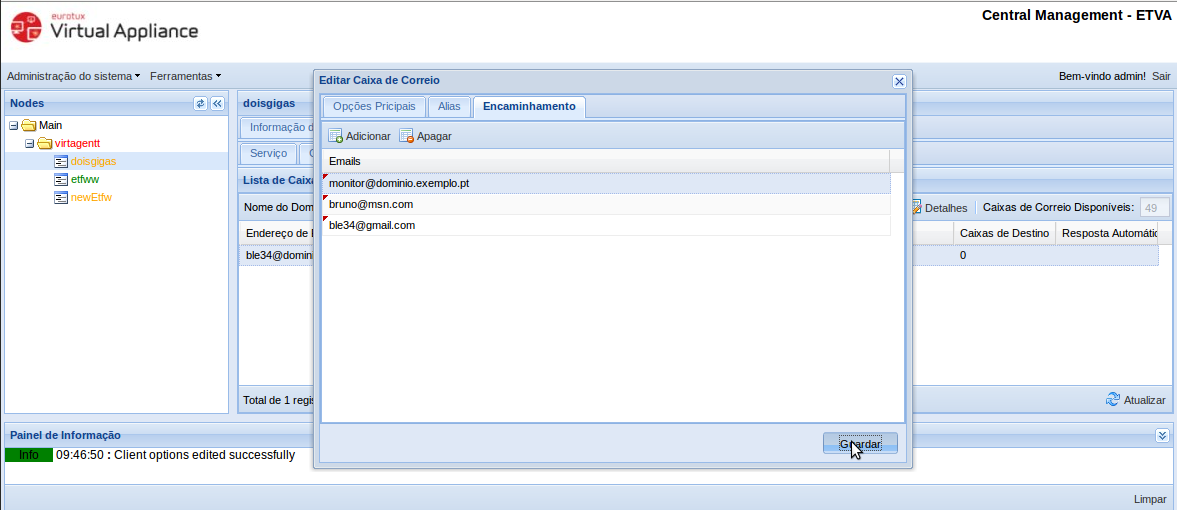
\includegraphics[scale=0.35]{screenshots/etms/etms_forwarding_mb_del.png}
    \caption{Definir Endereços para Encaminhamento de Emails}
    \label{fig:etms_forwarding_mb_del}
    \end{center}
\end{figure}

A remoção de caixas de encaminhamento é análogo à remoção de alias, bastando seleccionar o email em questão e escolher a opção \textit{Apagar}. Seleccionar \textit{Guardar} para que as alterações tenham efeito (procedimento análogo ao descrito em \ref{sec:etms_sub_alias_caixas_correio}).

\subsubsection{Caixas de Correio Disponíveis}
\label{sec:etms_sub_disponiveis_caixas_correio}
No caso em que o domínio pesquisado possua um limite de número de caixas de correio, aparece sobre o canto direito do separador, o número de caixas que ainda pode ser criado (ver imagem \ref{fig:etms_free_mb}). Este valor sofre um decremento após a criação de novas caixas, desabilitando a opção que possibilita a criação de novas caixas de correio quando o número de caixas de correio iguala/excede o limite definido.

\begin{figure}[H]
    \begin{center}
    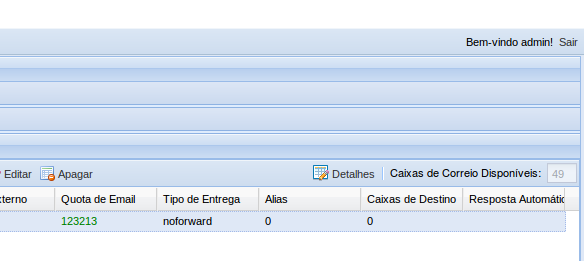
\includegraphics[scale=0.4]{screenshots/etms/etms_free_mb.png}
    \caption{Caixas de Correio Disponveis}
    \label{fig:etms_free_mb}
    \end{center}
\end{figure}


\subsubsection{Opção Detalhes}
\label{sec:etms_sub_detalhes_caixas_correio}
A opção \textit{Detalhes}, pertencente à barra de ferramentas que se encontra sob a \textit{Lista de Caixas de Correio} (à direita). Ao seleccionar esta opção são acrescentadas duas colunas à grelha que lista as caixas de correio, com informação relativa ao espaço ocupado pelas mensagens recebidas lidas e por ler (ver imagem \ref{fig:etms_mb_space}). Note que, por se tratar de uma operação computacional intensiva e potencialmente demorada, ao efectuar outro tipo de operações a coluna desaparece. Assim, sempre que se pretender actualizar/ver o espaço em disco ocupado, deve utilizar-se esta opção. No caso em que novas caixas de correio sejam acrescentas, o valor não aparece, tal acontece devido ao facto das directorias que armazenam os emails ainda não terem sido criadas.

\begin{figure}[H]
    \begin{center}
    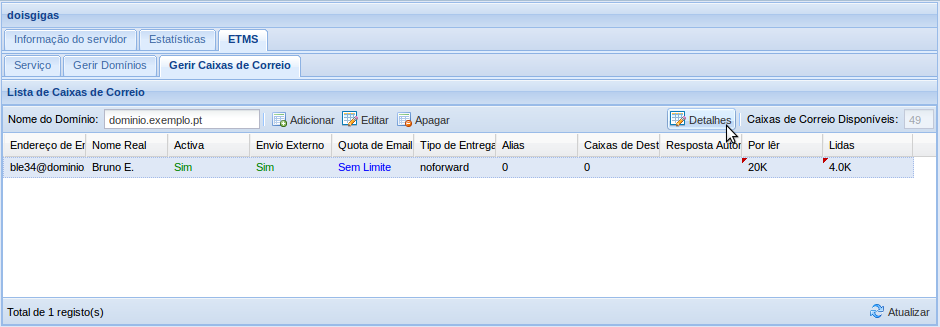
\includegraphics[scale=0.35]{screenshots/etms/etms_mb_space.png}
    \caption{Espaço Ocupado pelos Email da Caixas de Correio}
    \label{fig:etms_mb_space}
    \end{center}
\end{figure}



\subsubsection{Remoção de uma Caixa de Correio}
\label{sec:etms_sub_apagar_caixas_correio}
A remoção de uma caixa de correio, para além de remover todas as configurações, elimina todos os emails existentes nessa conta, não sendo possível recupera-los através do processo de restauro de configurações. Para proceder à remoção de conta, efectuar a pesquisa pelas caixas de correio do domínio \ref{sec:etms_sub_pesquisar_caixas_correio}, seleccionar a linha a que corresponde o caixa de correio, escolher a opção apagar e responder afirmativamente à mensagem de confirmação (imagem \ref{fig:etms_mb_del}).

\begin{figure}[H]
    \begin{center}
    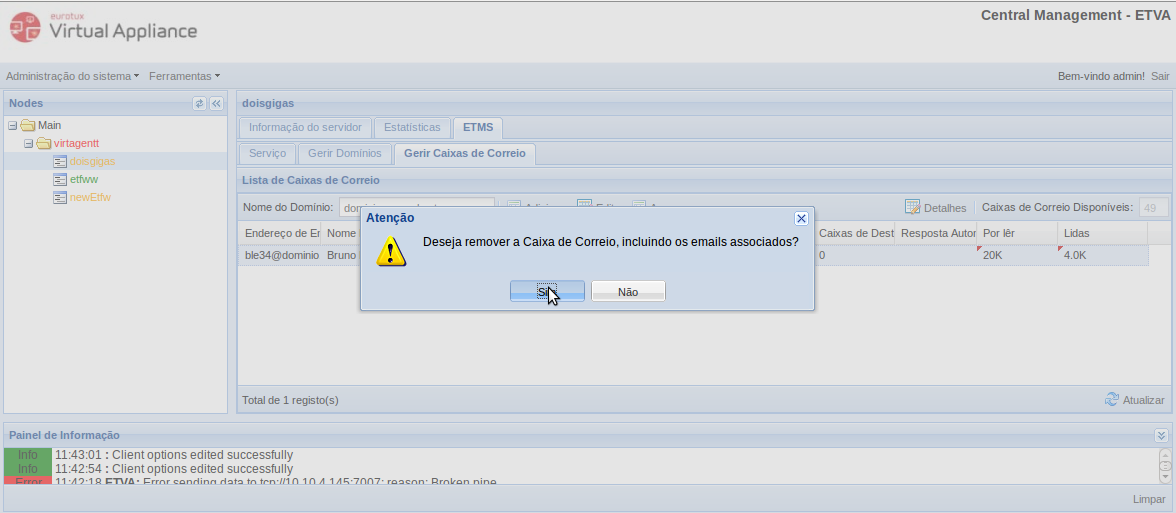
\includegraphics[scale=0.35]{screenshots/etms/etms_mb_del.png}
    \caption{Confirmar Eliminação da Caixa de Correio}
    \label{fig:etms_mb_del}
    \end{center}
\end{figure}
